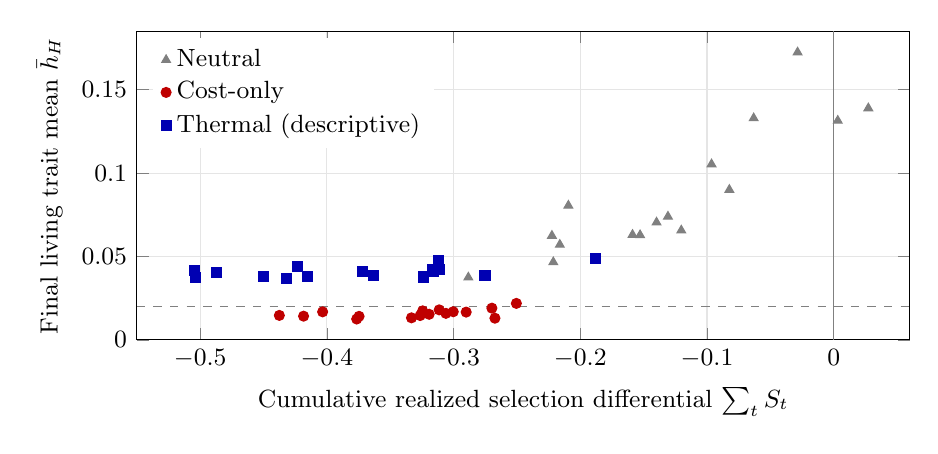
\begin{tikzpicture}
\begin{axis}[width=0.94\linewidth,height=5.5cm,
xmin=-.55,xmax=.06,ymin=0,ymax=.185,grid=major,grid style={gray!20},
xlabel={Cumulative realized selection differential $\sum_t S_t$},
ylabel={Final living trait mean $\bar h_H$},
scaled ticks=false,xtick={-.5,-.4,-.3,-.2,-.1,0},ytick={0,.05,.10,.15},
tick label style={font=\small,/pgf/number format/fixed,/pgf/number format/precision=2},label style={font=\small},
legend style={at={(0.02,0.98)},anchor=north west,font=\small,draw=none,fill=white},
legend cell align=left]
\addplot[gray,dashed,forget plot] coordinates {(-.55,.02) (.06,.02)};
\addplot[gray,thin,forget plot] coordinates {(0,0) (0,.185)};
\addplot[only marks,mark=triangle*,mark size=1.8pt,color=gray] coordinates {(-0.139818022077,0.070429589482) (0.003197024208,0.131463857067) (-0.028512073245,0.172426952121) (-0.152813675111,0.062846378957) (-0.222381500193,0.062479295953) (-0.209400339049,0.080557729662) (-0.096420667349,0.105335385432) (-0.082363983611,0.090031242368) (-0.120299457667,0.065668955443) (-0.221306800129,0.046614103389) (-0.158768564303,0.063038979682) (0.027318923874,0.138918112775) (-0.130812224143,0.073972515342) (-0.216146481562,0.057087908305) (-0.288353200405,0.037468018698) (-0.063161062301,0.132939407193)};
\addlegendentry{Neutral}
\addplot[only marks,mark=*,mark size=1.8pt,color=red!75!black] coordinates {(-0.437517913729,0.014690690714) (-0.290063122357,0.016678620873) (-0.324399220227,0.017421828001) (-0.267367204011,0.013026695039) (-0.333224063419,0.013241377855) (-0.311352049578,0.018020468349) (-0.403344729879,0.016837919428) (-0.326387180183,0.014604438182) (-0.376460943344,0.012525790739) (-0.319288908514,0.015373469051) (-0.418390635937,0.014242389554) (-0.269757896036,0.019037105658) (-0.250451154738,0.021894541789) (-0.306062293829,0.015930432347) (-0.300254467690,0.016890751352) (-0.374598367933,0.014137578112)};
\addlegendentry{Cost-only}
\addplot[only marks,mark=square*,mark size=1.8pt,color=blue!70!black] coordinates {(-0.316861419585,0.041986337362) (-0.449885653400,0.038041966359) (-0.275188336394,0.038861011146) (-0.432187789893,0.036802791130) (-0.312091856241,0.047502588176) (-0.323955178205,0.037707517642) (-0.415315043130,0.037823387289) (-0.503852087537,0.037266009481) (-0.315689088942,0.041092001237) (-0.188213936606,0.048786990046) (-0.311087230740,0.042346944600) (-0.504197931540,0.041538804381) (-0.423267591115,0.044054932914) (-0.487050076212,0.040681099994) (-0.371597304798,0.040885629219) (-0.363535771005,0.038507721260)};
\addlegendentry{Thermal (descriptive)}
\end{axis}
\end{tikzpicture}
